%!TEX root = paper.tex

%\section{Sampling} % (fold)
\section{Data Collection} % (fold)
\label{sec:sampling}

The goal of data collection is to collect sample variable valuations, based on which we can learn candidate invariants. In general, the more samples we have, the more likely we would learn the right invariants. However, if we simply learn based on the random samples, it may take many random samples before a classification algorithm can find the right invariant. In this work, we collect samples in three different ways: \emph{random sampling}, \emph{selective sampling} based on active learning and \emph{sampling through verification}. In the following, we discuss how each one works.

%Sampling is non-trivial in automatic loop invariant inference,
%because we need to obtain samples that are helpful for invariant candidate generation and refinement.
%Meanwhile, we can only ask whether a certain sample is in the invariant or not,
%without knowing the exact shape of the invariant.
%In order to face different sampling scenarios,
%we provide three different sampling approaches in this work:
%%we sample the program initial states in three different approaches:
%\emph{random sampling}, \emph{selective sampling} and \emph{counter-example sampling}.

%\begin{definition}[State]
%A state of a loop program execution, denoted as $s$, is an evaluation of the program variables at the loop condition checking position during that execution.
%\end{definition}
%\begin{definition}[Trace]
%In one program's execution, the program states at several locations compose one program trace.
%A trace of a loop program execution, denoted as $\langle s_0, s_1, ..., s_n\rangle$, is all the states of that execution which was reached one by one.
%\end{definition}
%
%Generally, our framework generates program initial states by sampling techniques and
%then execute the program from these states to collect traces and gather the program execution information at runtime.
%Later we propose a labeling method for the collected trace
%based on their satisfactions of $\mathit{Pre}$ and $\mathit{Post}$ during the execution.
%Generally, the sampling stage aims at obtaining samples with a high possibility to
%accurately generate the loop invariant so that the program specification can be verified.
%In order to face different sampling scenarios,
%we first provide three different sampling approaches.
%Then, we propose a labeling method for collected samples
%based on their satisfactions of $\mathit{Pre}$ and $\mathit{Post}$ conditions in the program.
% Before learning procedure, we need to gather some data from program.
% In a broader view, our framework is a kind of dynamic program verification approaches,
% thus it is quite interested in program execution states.
% Sampling is a way to tell the preference of program states.
% So in this step, we would like to sample a state with a high possibility
% if it is important for the learning afterwards.
% Then we execute program from these samples to gather more data
% and label them according to the satisfiability of $Pre$ and $Post$.
%, either randomly or using tools based on the idea of concolic testing~\cite{},

Random sampling provides us the initial set of samples to learn the first classifier. In this work, we have two ways to generate random samples. One is that we generate random values for each variable in $V$ based on its domain, assuming a uniform probabilistic distribution over all values in its domain. The other is that we use an SMT solver~\cite{barrett2009satisfiability,de2008z3} to systematically generate valuations that satisfy $\mathit{Pre}$ as well as those that dissatisfies $\mathit{Pre}$. We remark that these two ways are complementary. On one hand, without using a solver, we may not be able to generate valuations which satisfy $\mathit{Pre}$ if $\mathit{Pre}$ is very restrictive (or dissatisfy $\mathit{Pre}$ if the negation of $\mathit{Pre}$ is very restrictive). On the other hand, using a solver often generates biased valuations. We remark that the cost of generating a random sample is often negligible.

Anytime a classifier has been identified, we apply active learning and selective sampling to improve the classifier without applying heavy techniques like program verification.
The concept of active learning and selective sampling refers to the approaches that aim at reducing the effort of collecting and labeling samples (i.e., adding a sample into $\mathit{Positive}$, $\mathit{Negative}$ or $\mathit{NP}$ in our setting) by selecting only the most informative samples. Selective sampling methods have been proposed for different learning algorithms~\cite{DBLP:conf/icml/OrabonaC11}.
For instance, selective sampling techniques for SVM-based learning have been proven effective in achieving a
high accuracy with fewer examples in many applications~\cite{DBLP:conf/icml/OrabonaC11,DBLP:conf/mm/TongC01,DBLP:journals/jmlr/TongK01}.
The basic idea of selective sampling is that, given a classifier learned based on a set of samples, we calculate the most informative samples (according to the classifier) and label them so that the classifier can be improved the most.
For instance, in the setting of SVM, it has been proved that the most informative samples are those right on the classification boundary~\cite{DBLP:conf/icml/OrabonaC11}.
% Since an SVM classification function is represented
%by support vectors which are the samples closest to the boundary,
%this selective sampling effectively learns an accurate function with
%fewer labeled data [53]. In our setting, this means that we should
%generate a feature vector right by the classifier and applying program
%mutation and testing to label that feature vector so that the
%classifier would be improved.
%When we have a guess of loop invariants, we can apply selective sampling approach to finding more useful samples.
%Actually we apply this sampling method all along the learning procedure except the first iteration.
%\LL{I suggest do not use words like `obvious', nothing is obvious in a paper.}
%In fact, without labeled samples which are right on the boundary of the actual classifier,
%it is very unlikely that we would find it.
%Intuitively and intelligently, in order to get the `actual' classifier,
%we would require samples which would distinguish the actual one from any nearby one,
%This problem has been discussed and addressed in machine learning using active learning and selective sampling~\cite{DBLP:conf/icml/SchohnC00}.
%In our setting, this means that we should sample a program state right by the classifier and test the program
%with that state to label that feature vector so that the classifier would be improved.
%Algorithm~\ref{alg:active} presents details on how active learning is implemented in \textsc{Zilu}.
%At line 2, we obtain a classifier based on Algorithm~\ref{classify}.
%We compare the newly obtained classifier with the previous one at line 4, if they are identical, we return the classifier;
%otherwise we apply selective sampling so that we can generate additional labeled samples for improving the classifier.
%In particular, at line 5, we apply standard techniques~\cite{DBLP:conf/icml/SchohnC00} to select the most informative sample.
%Notice that in our setting, the most informative samples are those which are exactly on the lines and
%therefore can be obtained by solving an equation system.
%At line 8, we test the program with the newly generated samples so as to label them accordingly.
%After the above discussion, apparently the pre-requirement of selective sampling is there is a guess.
%In our setting, %after learning an candidate,
%which is usually a single polynomials or conjunction or \LL{disjunction?} of polynomials,
As a result, selective sampling can be reduced to solving an equation system based on the current classifier. We present details on how selective sampling is done with respects to two classification algorithms in the next section as examples. We remark that the selective sampling is often more expensive in time and memory than random sampling but cheaper than sampling through verification.


%In step 4, we add a small variance to variables because sometimes the points just lies on the boundary are very hard to tell their labels.
%\LL{this is however not clear how it is done.}
%As a result, this technique is applied all along the learning process except the very beginning.
%Counter-example sampling chooses samples lying in the difference zone between the invariant candidate and the actual invariant.
%Compared with the above sampling techniques, we should admit counter-example sampling is more directly and objective.
The last method of sampling is sampling through verification. When a candidate invariant fails any of the three conditions (1), (2) and (3) in the candidate verification stage,
a counter-example is provided by the verifier. We add the counter-example as new samples for the next learning iteration. We use the example shown in Figure~\ref{fig:running:example} to illustrate that sampling through verification is necessary. Assume that through random sampling, we have only obtained valuations in $\mathit{Positive}$ and $\mathit{NP}$ but never any in $Negative$. With selective sampling, we would converge to the half space separating $\mathit{Positive}$ and $\mathit{NP}$. As a result, we generate only one candidate invariant $x - y \geq 0$. During candidate verification, formula (6) is as follows. \[
x - y \geq 0 \land \neg (x < y) \land \neg (x \geq y \land x \leq y + 16)
\]
The formula is proven to be satisfiable, for instance, with a variable valuation $\{x \mapsto 17, y \mapsto 0\}$. According to our categorization, this valuation is added to $\mathit{Negative}$, which subsequently allow us to identify the candidate invariant separating $\mathit{Negative}$ from the rest: $x - y \geq 16$ and prove the Hoare triple.

%$\textsc{Zilu}$ tries to valid it using symbolic execution~\cite{king1976symbolic}\cite{khurshid2003generalized}
%(or known as concolic testing~\cite{sen2007concolic}) and constraint solving,
%which is shown in detail in Section ~\ref{sec:verification}.
%If it fails to validate, the constraint solver could provide us with counter-examples that can directly refute our invariant candidate.
%And as a result, it is quite useful for the invariant candidate refinement in the next learning procedure.
%\LL{This is oral language.
%Meanwhile, I do not understand what you are trying to say here. }
%As counter-example sampling technique sounds good, it seems this technique should be applied almost all the time,
%but the fact is it is applied only after failure of invariant candidate verification.
%That is because applying concolic testing and constraint solving is a more time-consuming job than the other two sampling methods.
% subsection sampling_approaches (end)

%This technique produce samples with the uniform distribution over a given range $\mathcal{R}$.
%It acts as an initialization sampling method
%as well as a supplementary sampling method in our framework.
%Firstly, before any classifier is learnt in our framework,
%we adopt simple random sampling solely to learn the initial candidate,
%which can be refined later in the invariant inference process.
%Secondly, the efficiency of other sampling methods, introduced in the following,
%depends largely on the similarity of the invariant candidate and the actual invariant.
%However, if the invariant candidate is very different from the correct invariant,
%random sampling can make the candidate converge faster than other sampling methods.
%Thirdly, since selective sampling can introduce biased samples distribution,
%random sampling aims at reducing its impact that can lead to a biased candidate result.
%As a result, the random sampling, as an important sampling approach,
%is applied to all the invariant inference iterations.
Figure~\ref{fig:sampling} visualizes how different sampling methods are related to each other in a 2-D plane. We start with the figure in the top-left corner. The (green) area above the line represents the space covered by the actual invariant. The dots are the samples obtained through random sampling. Based on these samples, a classifier is learnt to separate the random samples, as shown in the top-right figure. With this learnt invariant, selective sampling would us to identify those samples on the classification boundary based on the learnt classifier, as shown in the bottom-left figure. In comparison, sampling through verification would provide us the sample between the two lines shown in the bottom-left figure. It is obvious that the classifier will be improved with either selective sampling or sampling through verification, as shown in the bottom-right figure. The benefit of always applying selective sampling before applying sampling through verification is that verification is often more costly and thus we would like to avoid it as much as possible. \\

%the red area is the learnt invariant captured by the red line;
%the green nodes represent the samples inside of the correct invariant;
%and the red nodes represent the samples outside of the correct invariant.
%The random sampling is very useful in generating the initial invariant
%as well as searching for samples that cannot be reached
%by selective sampling and counter-example sampling.
%For instance, in Figure~\ref{fig:sampling:random},
%we obtain four samples using random sampling
%and learn the initial invariant in Figure~\ref{fig:sampling:random:invariant}.
%When an invariant has been learnt,
%we can accelerate the invariant convergence by obtaining samples that
%land exactly on the edges of the learnt invariant (i.e., selective sampling)
%or conflict the required properties (i.e., counter-example sampling).
%For example, in Figure~\ref{fig:sampling:selective},
%we select four samples on borders of the learnt invariant and
%compute one counter-example to help generating the real invariant.
%As can be seen in Figure~\ref{fig:sampling:selective:invariant},
%the newly learnt invariant moves towards the real invariant quickly.

\begin{figure}[t]
        \centering
        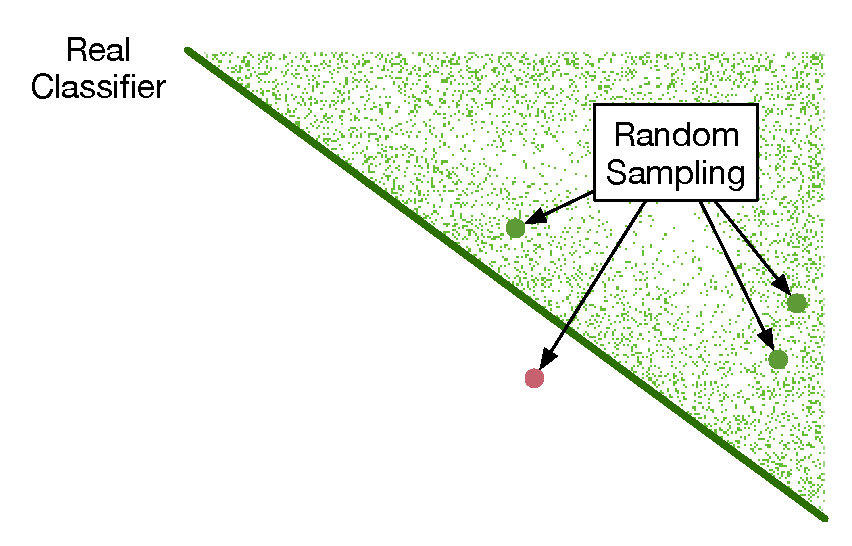
\includegraphics[scale=0.3]{figures/general-sampling-0.pdf}
%        \caption{Random Sampling}
        \centering
        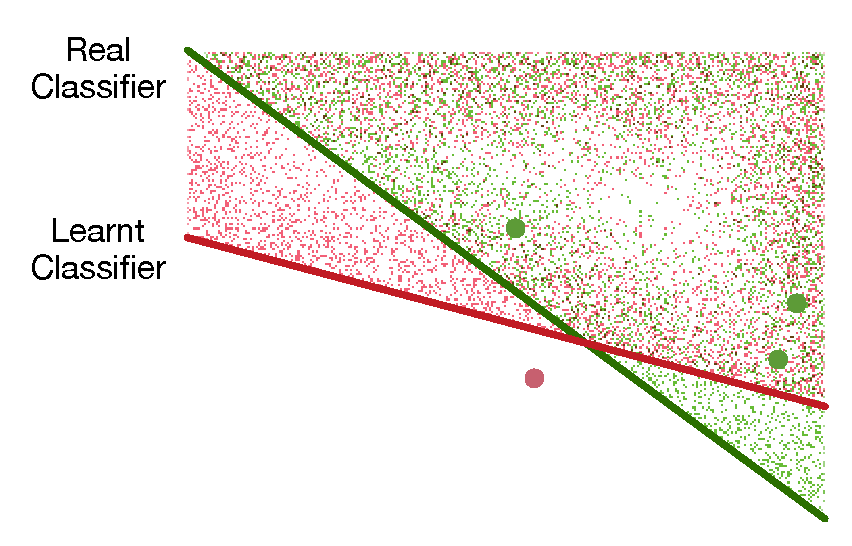
\includegraphics[scale=0.3]{figures/general-sampling-1.pdf} \\
%        \caption{Learnt Invariant}
        \centering
        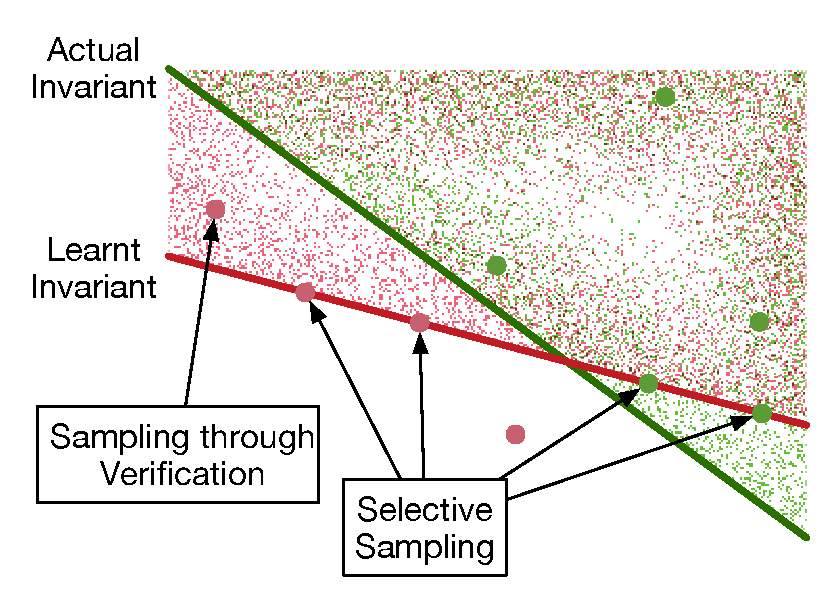
\includegraphics[scale=0.3]{figures/general-sampling-2.pdf}
%        \caption{Selective and Counter-Example Sampling}
        \centering
        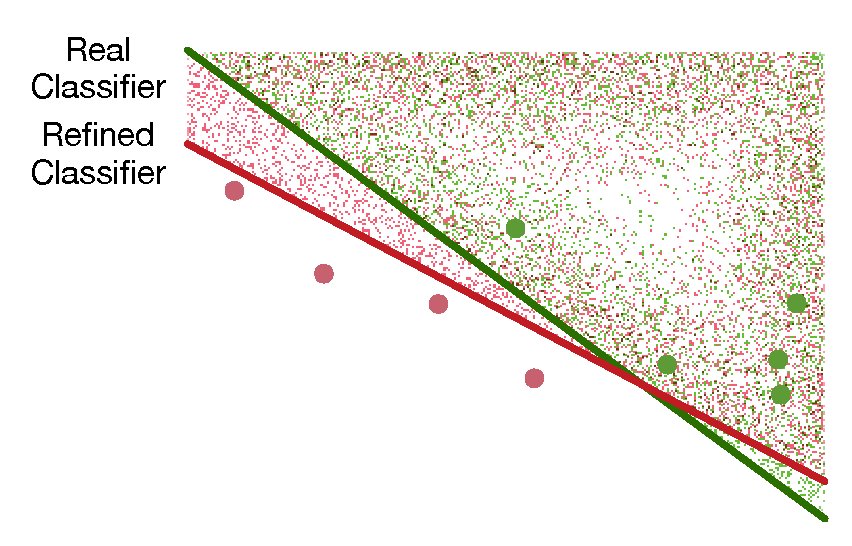
\includegraphics[scale=0.3]{figures/general-sampling-3.pdf}
%        \caption{Refined Invariant}
    \caption{Sampling approaches}
    \label{fig:sampling}
\end{figure}

\noindent
In the following, we define the four sets of samples formally. Let $\mathit{SP}$ be the set of samples we obtain (through any of the above-discussed sampling methods). For each sample $s_0 \in \mathit{SP}$, by executing the given program with the initial variable valuation $s_0$, we can obtain a sequence of variable valuation $\langle s_0, s_1, \cdots, s_n \rangle$ where $s_i = \mathit{Body}^i(s_0)$ and $s_n \not \models \mathit{Cond}$ and $s_k \models \mathit{Cond}$ for all $0 \leq k < n$. In the following, we write $s \Rightarrow s'$ to denote that: either $s' = s$ or there exists $i$ such that $Body^i(s) = s'$ and $Body^k(s) \models Cond$ for all $k$ such that $0 \leq k < i$, i.e., executing the program with the initial variable valuation $s$, we could have the variable valuation $s'$ after some number of iterations.
% there exists a sample $s_0 \in \mathit{Sample}$ and a corresponding sequence of variable valuation $\langle s_0, \cdots, s_i, \cdots, s_j, \cdots s_n \rangle$ such that $s_i = s$ and $s_j = s'$.
Next, we define the four disjoint sets of samples as follows.
\[
\mathit{CE}(\mathit{SP}) = \{s | \exists s_0 \in SP.~s_0 \Rightarrow s \Rightarrow s_n \land s \models Pre \land s_n \not \models Cond \land s_n \not \models \mathit{Post}\} \]
$CE(SP)$ is the set of valuations such that a valuation in $CE(SP)$ satisfies $Pre$ and becomes a valuation $s_n$ which fails $Post$ when the loop terminates. We remark that a valuation in $CE(SP)$ may be a valuation in $SP$ or one which can be reached from one in $SP$ after some iterations. If $\mathit{CE}(\mathit{SP})$ is non-empty, the Hoare triple is disproved.
\begin{align*}
 \mathit{Positive}(\mathit{SP}) = & \{s | \exists s_0 \in SP.~\exists s'.~s_0 \Rightarrow s' \Rightarrow s \Rightarrow s_n \land \\
     & ~~~~~~s' \models \mathit{Pre} \land s_n \not \models Cond \land s_n \models \mathit{Post}\}
\end{align*}
%\[
% \mathit{Positive}(\mathit{SP}) = \\
%~~~~~~\{s | \exists s_0 \in SP.~\exists s'.~s_0 \Rightarrow s' \Rightarrow s \Rightarrow s_n \land s' \models \mathit{Pre} \land s_n \not \models Cond \land s_n \models \mathit{Post}\}
% \]
$Positive(SP)$ is the set of valuations such that a valuation $s$ in $Postive(SP)$ can be reached by a valuation satisfying $Pre$ and $s$ becomes a valuation $s_n$ which satisfies $Post$ when the loop terminates. We show that any $s$ in $Positive(SP)$ must satisfy $Inv$. Because $s' \models Pre$, $s' \models Inv$ since $\mathit{Inv}$ satisfies condition (1). Since $\mathit{Inv}$ satisfies condition (2) and $Body(s') \models Inv$ if $Body(s') \models Cond$. Since $s = Body^i(s')$ for some $i$ and by definition $Body^j(s') \not \models Cond$ for all $j \leq i$, we have $s \models Inv$.
 \[
    \mathit{Negative}(\mathit{SP}) = \{s | \exists s_0 \in SP.~s_0 \Rightarrow s \Rightarrow s_n \land s \not \models \mathit{Pre} \land s_n \not \models Cond \land s_n \not \models Post\} \]
$Negitive(SP)$ is the set of valuations such that a valuation $s$ in $Negitive(SP)$ fails $Pre$ and becomes a valuation $s_n$ which fails $Post$ when the loop terminates. We show that $s \not \models \mathit{Inv}$ for all $\mathit{Inv}$ satisfying condition (1), (2) and (3). Assume that $s \in Inv$, by condition (2), we can show that $s_n$ must satisfy $Inv$ through a simple induction. By condition (3), $s_n$ must satisfy $post$, which contradicts the definition of $Negitive(SP)$.
\[    \mathit{NP}(\mathit{SP}) = \{s | \exists s_0 \in SP.~ s_0 \Rightarrow s \land s \not \in CE(SP) \cup Positive(SP) \cup Negative(SP)\}
\]
$NP(SP)$ is the set of valuations which are not in any of the three sets defined above. We remark that a valuation $s$ in $NP(SP)$ may or may not satisfy an $Inv$ which satisfies condition (1), (2) and (3).

%\subsection {Loop Execution}
%With the initial states $\mathcal{S}$ obtained above,
%we execute the program from the state $s$ in $\mathcal{S}$.
%From program execution,
%we can generate more program states and check their satisfiability to $Pre$ and $Post$.
%%In this step,
%%we execute the program from the initial state $s_0$, where $s_0 \in \mathcal{S}$ and $\mathcal{S}$ is obtained from the above technique.
%A trace $\langle s_0, s_1, ..., s_i, ..., s_n\rangle$ in a loop program is called a loop trace,
%if $s_0$ is the initial state before entering the loop,
%$s_i$ is the state just after executing loop $Body$ for $i$ times,
%and $s_n$ is the state satisfying $\neg B$ and thus the execution jumps out the loop $Body$.
%
%We record the execution trace $\langle s_0, s_1, ..., s_i, ..., s_n\rangle$ with the satisfaction to $Pre$ and $Post$.
%%\begin{itemize}
%%\item Trace $\langle s_0, s_1, ..., s_i, ..., s_n\rangle$
%%\item $s_0 \models Pre$ or $s_0 \models \neg Pre$;
%%\item $s_n \models Post$ or $s_n \models \neg Post$.
%%\end{itemize}
%For example, if we start the program execution with the sample $\{(x,y) \mapsto (3, 12)\}$ from the last selective sampling,
%we could record a trace $\mathcal(t) = \langle (3, 12), (13, 15), (23, 18)\rangle$ and $s_0 \models Pre$, $s_2 \models Post$.
%
%
%\subsection{Labeling} % (fold)
%\label{sub:labeling}
%
%%\LL{I feel the labeling and sampling described here are inaccurate.
%%Sampling should include all of the samples rather than only the initial inputs.
%%We can discuss later. }
%%With the samples $S$ obtained above, we execute the program with initial state $s$ in $S$.
%%\LL{Here, the initial state is unclear. what is program state. }
%%From program execution, we can generate more program states and check their satisfiability to $Pre$ and $Post$.
%%In this step, we present the technique how we label them according to these information.
%
%To demonstrate the technique, a few symbols should be introduced first.
%$Body(s)$, defined in Section~\ref{sec:introduction}, is the state which could be reached after executing $Body$ from state $s$.
%$Body^*(s)$ denotes the set of program states which could be reached after executing zero or more iterations of the loop starting from $s$.
%Furthermore, we write $s \multimap s'$ to denote that starting with a program state $s$ would result in state $s'$ when the loop terminates.
%%\LL{I suggest use $\rightarrow$, $\rightarrow^*$ and $\multimap$. }
%%\LL{What is Trace, defined?}
%So if there is an execution trace $\langle s_0, s_1, ..., s_i, ..., s_n\rangle$
%%$Trace\{s_0 \to s_1 \to ...\to s_i \to ... \to s_n\}$,
%%where $s_0$ is the initial state before entering the loop,
%%$s_i$ is the state just after executing loop $Body$ for $i$ times,
%%and $s_n$ is the state satisfying $\neg B$ and thus the execution jumps out the loop $Body$,
%then we have
%\begin{itemize}
%\item $s_{i+1} = Body(s_i)~~~~\forall i \in [0, \ldots, n-1]$.
%\item $s_{i} \in Body^*(s_0)~~~~~~\forall i \in [0, \ldots, n]$.
%\item $s_{0} \multimap s_{n}$.
%\end{itemize}
%%We write $Body^*(S)$ to denote $\{s' | \exists s \in S \cdot s' \in Body^*(s)\}$.
%
%According to the satisfactory of the loop invariant,
%we category program states into two classes:
%positive states, which means the states satisfy the loop invariant;
%and negative states, which means the states do not satisfy the loop invariant.
%\begin{definition}[Positive State]
%Positive state is a state of the loop execution that satisfy the loop invariant.
%\end{definition}
%\begin{definition}[Negative State]
%Negative state is a state of the loop execution that does not satisfy the loop invariant.
%\end{definition}
%
%\begin{theorem}
%If an execution trace $\mathcal{T} = \langle s_0, s_1, ..., s_n\rangle$ satisfies $s_0 \models Pre$ and $s_n \models Post$,
%then all the states in $\mathcal{T}$ are positive states.
%\end{theorem}
%
%%\begin{proof}[Proof of the Main Theorem]
%From constraint~\ref{inv:pre}, for an invariant $Inv$,
%any state satisfying $Pre$ should also satisfies $Inv$.
%Therefore, $s_0$ is a postive state.
%
%From constraint~\ref{inv:loop}, $s_1$ is a positive state, as $s_0 \models Inv$
%and  $s_0 \models Cond$ (because $s_0 is not the last state in the trace$);
%then $s_i~~\forall i \in [0...n]$ is a positive state due to the induction.
%
%Therefore, all the states in $\mathcal{T}$ are positive states. \hfill \qed
%%\end{proof}
%
%
%
%\begin{theorem}
%If an execution trace $\mathcal{T} = \langle s_0, s_1, ..., s_n\rangle$ satisfies $s_0 \models \neg Pre$ and $s_n \models \neg Post$,
%then all the states in $\mathcal{T}$ are negative states.
%\end{theorem}
%From constraint~\ref{inv:post}, for an invariant $Inv$,
%$s_n$ not satisfying $Post$ can infer $s_n \models \neg(Inv \wedge \neg Cond)$.
%As $s_n$ is the last state in trace $\mathcal{T}$, $s_n \models \neg Cond$, and thus $s_n \models \neg Inv$.
%Therefore, $s_n$ is a negative state.
%
%From constraint~\ref{inv:loop}, $s_{n-1}$ is a negative state, as $s_n \models \neg Inv$ and $s_{n-1} \models Cond$;
%then $s_i~~\forall i \in [0...n]$ is a negative state due to the induction.
%
%Therefore, all the states in $\mathcal{T}$ are negative states. \hfill \qed
%
%
%\begin{theorem}
%If an execution trace $\mathcal{T} = \langle s_0, s_1, ..., s_n\rangle$ satisfies $s_0 \models Pre$ and $s_n \models \neg Post$,
%then $\mathcal{T}$ is a counter-example trace which can disprove the program specification.
%\end{theorem}
%
%If the program specification is correct,
%we can prove all the states in $\mathcal{T}$ are positive states as theorem 2.
%Using constaint~\ref{inv:post}, we can get $s_n \models Post$, which violates the assumption here.
%
%Therefore, $\mathcal{T}$ is a counter-example trace which can disprove the program specification. \hfill \qed
%
%\begin{definition}[Implication Trace]
%An implication trace $\mathcal{T} = \langle s_0, s_1, ..., s_n\rangle$ satisfies if $s_i \models \mathcal{I} \rightarrow s_{i+1} \models \mathcal{I} ~~\forall i \in [0, 1, ..., (n-1)]$.
%\end{definition} \hfill \qed
%
%\begin{theorem}
%If an execution trace $\mathcal{T} = \langle s_0, s_1, ..., s_n\rangle$ satisfies $s_0 \models \neg Pre$ and $s_n \models Post$,
%then $\mathcal{T}$ is an implication trace.
%\end{theorem}
%From constraint~\ref{inv:loop}, we know this is true. \hfill \qed
%
%
%
%
%In total , we can categorize all the program traces
%% $Body^*(S)$
%started from Set $S$ into four sets according to the following table.
%In the Table~\ref{tab:labeling}
%$\mathcal{S}^\chi$ stands for counter-example trace;
%$\mathcal{S}^+$ stands for traces with all the positive states;
%$\mathcal{S}^-$ stands for traces with all the negative states;
%and $\mathcal{S}^\rightarrow$ stands for implication traces.
%
%%They can be judged according to Table~\ref{tab:labeling}:
%\begin{table}[htb]
%\centering
%\begin{tabular}[float]{|c|c|c|}
%\hline
%$\mathcal{T} = \langle s_0, s_1, ..., s_n\rangle$ & $s_n \models Post$            & $s_n \models \neg Post$\\
%\hline
%$s_o \models Pre$                 & $\mathcal{T} \in \mathcal{S}^+$       		  & $\mathcal{T} \in \mathcal{S}^\chi$\\
%\hline
%$s_0 \models \neg Pre$            & $\mathcal{T} \in \mathcal{S}^\rightarrow$     & $Body^*(s_0) \in \mathcal{S}^-$\\
%\hline
%\end{tabular}
%\caption{Trace Labeling Table}
%\label{tab:labeling}
%\end{table}
%
%In our framework, these traces are used in different ways:
%positive states and negative states can be used to learn classifiers directly,
%which will be shown in Section~\ref{sec:learning};
%Counter example traces can be used to validate program specification:
%our framework terminates execution immediately when it meets a counter example trace.
%Implication traces can be applied to validating a learned classifier,
%For instance, providing a candidate $\mathcal{C} = x - y \ge 0$ and an implication trace
%$\langle s_0, s_1, s_2\rangle$where
%$$s_0 = \big(x \mapsto 2, y \mapsto 1\big),  s_1 = \big(x \mapsto 2, y \mapsto 2\big),  s_2 = \big(x \mapsto 2, y \mapsto 3\big),$$
%we could refute this candidate instantly.
%For using $\mathcal{C}$ to label this whole trace as $$s_0 \mapsto +,  s_1 \mapsto +,  s_2 \mapsto -,$$
%we find this violates the above implication rules,
%indicating the current candidate $\mathcal{C}$ must be not an actual invariant.









%\medskip\noindent
%\textbf{Positive State, Negative State and Implication Pair}
%are three concepts are originally introduced in \cite{sharma2014invariant}.
%They tell whether a state must satisfy the loop invariant or must not.
%A positive state is a state that must satisfy the actual loop invariant,
%while a negative state is a state that must not satisfy the invariant.
%An implication pair is a pair of state, the latter one satisfying the invariant
%if the former one satisfies it.
%In this part, we demonstrate the rules to category a state according to its execution information.
%\LL{I feel you do not need to put them as a section (I mean that it should not look like above).
%Say the positive states and the positive trace together.}


%From constraint~\ref{inv:pre} we know, for an invariant $Inv$,
%any state satisfying $Pre$ should also satisfies $Inv$.
%Therefore, the state satisfying $Pre$ must be a positive state.
%\LL{Why do you want to say that it must be a positive state?}

%\LL{The following is extremely hard to understand (grammar error).
%Give definition first, purpose later.}
%The adjacent states $(s, t)$ appeared in a trace a pair of states is an implication pair,
%because, according to the inductive property~\ref{inv:loop},
%$(s \models Inv) \Rightarrow (t \models {Inv})$
%if $t = Body(s)$ and $s \models Cond$.
%On the contrary, for an invariant candidate $\mathcal{C}$,
%if there is an implication $(s, t)$ in which $(s \models \mathcal{C}) \wedge (t \models \neg \mathcal{C})$,
%$\mathcal{C}$ is proved to be an invalid invariant.

%Finally, a state satisfying $\neg{Cond} \wedge \neg{Post}$ must be a negative state.
%Considering constraint~\ref{inv:post}, if a state $s \models \neg{Post}$,
%then $s \models \neg(Inv \wedge \neg Cond)$.
%In this situation $s \models \neg Cond$, then we can infer $s \models \neg Inv$.

%\medskip\noindent
%\textbf{Positive Trace, Negative Trace, Implication Trace.}
%\LL{Change above, do not put them as a section title.}
%As an execution trace contains more data than a single state,
%this part discusses the technique to label all the states in one trace at a time rather than just a single state.
%Similar to the state labeling, a positive trace defines a trace with all positive states,
%while a negative trace defines a trace with all negative states.
%An implication trace is a trace in which, if one state is the positive state,
%all the states afterwards are positive states.
%We state the regulation to determine the class of any given trace as follows.

%For a trace $Trace\{s_0 \to s_1 \to ... \to s_i \to ... \to s_n\}$,
%if $s_0 \models Pre$, and $s_n \models Post$,
%then this is a positive trace, meaning $\forall s_i \models Inv$.
%Because if state $s_0$ satisfy $Pre$,
%$s_0$ is a positive state that must satisfy $Inv$. %, according to equation 1.
%Considering constraint~\ref{inv:loop}, $s_1$ is also positive states.
%Then all the states in $Trace\{s_0 \to s_1 \to ...\to s_i, ... \to s_n\}$ are positive states inductively.
%So now we can get a positive trace  $Trace\{s_0 \to s_1 \to ...\to s_i \to ... \to s_n\}$.

%On the contrary, for a trace $Trace\{s_0 \to s_1 \to ...\to s_i \to ... \to s_n\}$,
%if $s_0 \models \neg Pre$, and $s_n \models \neg Post$,
%we can infer this is a negative trace in the similar way.

%The third case is a trace that begins with a state $s_0 \models Pre$ and ends with a state $s_n \models \neg Post$,
%\LL{obviously}, this is a counter-example to disprove the program and its specification.
%As a result, if $\textsc{Zilu}$ meets any counter-example trace in the testing,
%the execution exits immediately with a failure message indicating a bug in the program.

%The last case is a trace begin with a state $s_0 \models \neg Pre$ but ends with a state $s_n \models Post$.
%Under this condition, we could not determine whether $s_0$ and $s_n$ satisfy invariants or not,
%not to mention other states $\{s_1, s_2, ..., s_{n-1}\}$.
%Then this trace belongs to the implication trace set, meaning if $s_i \models Inv$, then $s_j \models Inv$ $\forall j \ge i$.
%Implication traces can not be used to learn classifiers directly,
%however, they have power in validating a candidate.
%For instance, providing a candidate $\mathcal{C} = x - y \ge 0$ and an implication trace
%$\langle s_0, s_1, s_2\rangle$where
%$$s_0 = \big(x \mapsto 2, y \mapsto 1\big),  s_1 = \big(x \mapsto 2, y \mapsto 2\big),  s_2 = \big(x \mapsto 2, y \mapsto 3\big),$$
%we could refute this candidate instantly.
%For using $\mathcal{C}$ to label this whole trace as $$s_0 \mapsto +,  s_1 \mapsto +,  s_2 \mapsto -,$$
%we find this violates the above implication rules,
%indicating the current candidate $\mathcal{C}$ must be not an actual invariant.

% subsection labeling (end)

% section sampling (end)
